\documentclass[12pt,a4paper]{report}

% --- Packages ---
\usepackage[utf8]{inputenc}
\usepackage[T1]{fontenc}
\usepackage[english]{babel}
\usepackage{geometry}
\geometry{a4paper, portrait, margin=1.5cm}
\usepackage{graphicx}
\usepackage{hyperref}
\usepackage{listings}
\usepackage{xcolor}
\usepackage{booktabs}
\usepackage{enumitem}
\usepackage{amsmath}
\usepackage{titlesec}
\titleformat{\chapter}[hang]{\normalfont\huge\bfseries}{\thechapter}{1em}{}
\titlespacing*{\chapter}{0pt}{-20pt}{20pt}
\usepackage{caption}
\usepackage{float}
\usepackage{amssymb}
\usepackage{pifont}
\usepackage{tabularx}
\usepackage{array}

% --- Code Listing Style ---
\definecolor{codebg}{rgb}{0.95,0.95,0.95}
\definecolor{codegreen}{rgb}{0.25,0.49,0.48}
\definecolor{codegray}{rgb}{0.5,0.5,0.5}
\definecolor{codepurple}{rgb}{0.58,0,0.82}

\lstset{
    backgroundcolor=\color{codebg},
    basicstyle=\ttfamily\footnotesize,
    breaklines=true,
    captionpos=b,
    commentstyle=\color{codegreen},
    keywordstyle=\color{blue},
    stringstyle=\color{codepurple},
    numberstyle=\tiny\color{codegray},
    numbers=left,
    frame=single,
    rulecolor=\color{black!30},
    tabsize=4,
    showstringspaces=false,
}

\lstdefinestyle{kernel}{
    language=C,
    morekeywords={uint64_t,uint32_t,int32_t,u64,u32,u16,u8,s64,s32,bool,
                  struct,enum,static,inline,__u8,__u32,__u64},
}

\lstdefinestyle{log}{
    basicstyle=\ttfamily\scriptsize,
    numbers=none,
    frame=single,
    backgroundcolor=\color{black!5},
}

% --- Header/Footer ---
\pagestyle{plain}

% --- Title ---
\begin{document}
\begin{titlepage}
    \center

    \begin{figure}[h!]
        \centering
        
\includegraphics[width=.5\linewidth]{resources/logo1.jpg} \\
        
\includegraphics[width=.5\linewidth]{resources/logo2.jpg} \\
    \end{figure}

    \vspace*{2em}

    \rule{\linewidth}{.1em}
    \\[1em]
    {\huge\bfseries eBPF: Verifier Vulnerabilities and Exploitation}
    \\[.33em]
    \rule{\linewidth}{.1em}
    \\[2em]
    
    \Large
    \textbf{Andrea Botticella s347291} \\
    \vspace{0.5em}
    \large
    Politecnico di Torino \\
    Security Verification and Testing \\
    eBPF Research Lab \\
    \vspace{2em}
    
    \vfill
    \large \today
\end{titlepage}
\thispagestyle{empty}

% \begin{abstract}
% \input{sections/abstract.tex}
% \end{abstract}

\tableofcontents
\newpage

\chapter{Introduction}

\section{eBPF Background}
Extended Berkeley Packet Filter (eBPF) allows user-space programs to safely execute custom logic inside the Linux kernel without needing custom modules. Because these programs run in ring-0, a single vulnerability could easily crash the system or lead to privilege escalation. To prevent this, every eBPF program must pass the \textbf{BPF verifier}, a static analysis engine inside the kernel that formally checks the program for memory safety and type correctness before JIT compilation. 

This report documents an analysis of four significant logic bugs affecting the verifier, comparing their root causes, exploitation primitives, and the protective mechanisms that mitigate them.

\section{Research Objectives}
This project is part of the Security Verification and Testing course. The main goal is to analyze the patches, understand the vulnerabilities at a deep technical level, and develop proof-of-concept code for several verifier CVEs. While there are many vulnerabilities available for study, I have selected the following ones for this research:
\begin{itemize}
    \item \textbf{CVE-2021-3600}: A 32-bit truncation bug during the verifier's div/mod instruction fixup, leading to bounds tracking confusion and Out-Of-Bounds (OOB) memory access.
    \item \textbf{CVE-2021-3444}: The sister bug of CVE-2021-3600, targeting the mod32 destination register truncation. Exploited on kernel 4.19.19 (where \texttt{alu\_limit} is absent) to achieve a \textbf{full unprivileged local privilege escalation} via ret2usr.
    \item \textbf{CVE-2023-52452}: An integer tracking flaw regarding variable-offset stack writes, which incorrectly calculates the depth of stack frames and causes stack corruption.
    \item \textbf{CVE-2024-26589}: A missing bounds check inside the restricted pointer arithmetic mechanisms which allows arbitrary offset-addition to the \texttt{flow\_keys} structures, leading to stack OOB.
\end{itemize}

\section{Research Methodology}
The exploitation process is organized into distinct, verifiable \textit{Milestones}, starting from initial vulnerability confirmation (such as information leaks) up to more advanced exploitation stages and analyzing the technical feasibility of different attack vectors. 

This modular structure ensures that the research methodology remains both robust and extensible for future vulnerability analyses, allowing for the seamless integration of additional CVE studies regardless of the specific subsystem or bug class involved.

\section{Common Experimental Framework}

To improve reproducibility and keep the methodology scalable as new CVEs are added, experiments are conducted using a shared framework and CVE-specific parameterization. This section defines what is common across analyses; concrete values (kernel release, config variants, and mitigation profile) are documented inside each CVE chapter.

\begin{table}[H]
\centering
\small
\begin{tabular}{@{}ll@{}}
\toprule
\textbf{Component} & \textbf{Common baseline} \\
\midrule
Build workflow & Buildroot-based pipeline orchestrated by project scripts \\
Virtualization & QEMU/KVM virtual testbed \\
Root filesystem strategy & Minimal Buildroot image with CVE overlays \\
Kernel strategy & Per-CVE vulnerable target kernel selected for validation \\
eBPF core requirements & \texttt{CONFIG\_BPF\_SYSCALL=y}, \texttt{CONFIG\_BPF\_JIT=y} \\
Debug and observability & Kernel symbols/debug options enabled when needed by the CVE \\
Mitigation profile handling & Controlled and documented per scenario (privileged/unprivileged) \\
Compiler/toolchain strategy & Static user-space binaries for deterministic VM execution \\
Execution model & Milestone-driven validation and incremental exploit development \\
\bottomrule
\end{tabular}
\caption{Shared experimental framework used across CVE analyses}
\end{table}

This separation between common framework and per-CVE specifics keeps the report coherent, extensible, and directly reusable for future verifier vulnerability studies.


\newpage
% CVE Sections
\chapter{CVE-2021-3600}

\section{CVE Selection}
I selected CVE-2021-3600 inspired by previous years' research projects, such as CVE-2020-8835, which pioneered scalar bounds confusion on BPF Maps. This case provides an architectural study of how post-verification instruction rewriting can undermine the safety proofs established by the verifier, and it allowed me to test how modern kernel mitigations, specifically the \texttt{alu\_limit} pointer arithmetic sanitization, respond to a classic bounds tracking mismatch between the verifier and the JIT compiler.

\section{Vulnerability Analysis}

\subsection{Root Cause}

The root cause lies in \texttt{fixup\_bpf\_calls()} in \texttt{kernel/bpf/verifier.c}. This function is a post-verification pass that rewrites certain BPF instructions before JIT compilation. For 32-bit division and modulo operations, the vulnerable code inserts:

\textbf{Vulnerable Code and Truncation Bug}

\begin{lstlisting}[style=kernel,caption={Vulnerable fixup code (kernel/bpf/verifier.c, fixup\_bpf\_calls())}]
struct bpf_insn mask_and_div[] = {
    BPF_MOV32_REG(insn->src_reg, insn->src_reg),  // BUG!
    /* Rx div 0 -> 0 */
    BPF_JMP_IMM(BPF_JNE, insn->src_reg, 0, 2),   // 64-bit jump!
    BPF_ALU32_REG(BPF_XOR, insn->dst_reg, insn->dst_reg),
    BPF_JMP_IMM(BPF_JA, 0, 0, 1),
    *insn,
};
\end{lstlisting}

\textbf{Why \texttt{BPF\_MOV32\_REG} is wrong:}
The \texttt{BPF\_MOV32\_REG(src, src)} instruction zeroes the upper 32 bits of the source register at \emph{runtime}. However, the verifier's abstract interpretation of the program happens \emph{before} \texttt{fixup\_bpf\_calls()} runs. The verifier never sees this inserted \texttt{mov32} instruction, so its bounds tracking for the source register remains unchanged, it still reflects the full 64-bit value.

Furthermore, during the actual \texttt{BPF\_\allowbreak ALU | BPF\_\allowbreak DIV | BPF\_\allowbreak X} verification, the function \texttt{adjust\_\allowbreak scalar\_\allowbreak min\_\allowbreak max\_\allowbreak vals()} only marks the \emph{destination} register as unknown after division, the source register's bounds are not updated.

\textbf{The double bug:}
There is actually a second problem: the zero-check \texttt{BPF\_JMP\_IMM(BPF\_JNE, src, 0, 2)} uses a \textbf{64-bit comparison}, even for 32-bit operations. After the \texttt{mov32} truncation, a value like \texttt{0xFFFFFFFF} (which is nonzero) would not trigger the zero-check. But the verifier, which still tracks the original 64-bit value, may compute the wrong result for the division.

\textbf{Concrete Example:}

\begin{lstlisting}[style=kernel,caption={Bounds mismatch demonstration}]
// Source level:
0: (b7) r0 = -1           // R0 = 0xFFFFFFFF_FFFFFFFF
1: (b7) r1 = -1           // R1 = 0xFFFFFFFF_FFFFFFFF
2: (3c) w0 /= w1          // 32-bit division

// After fixup_bpf_calls() rewrites instruction 2:
2a: (bc) w1 = w1          // mov32: R1 -> 0x0000_0000_FFFF_FFFF
2b: (15) if r1 == 0 goto  // 64-bit zero check (R1 != 0, so not taken)
2c: (3c) w0 /= w1         // actual division
\end{lstlisting}

\begin{table}[H]
\centering
\begin{tabular}{@{}lll@{}}
\toprule
\textbf{Register} & \textbf{Verifier State} & \textbf{Runtime Value} \\
\midrule
R1 before div & \texttt{0xFFFFFFFF\_FFFFFFFF} (-1) & \texttt{0x0000\_0000\_FFFF\_FFFF} (after mov32) \\
R1 >> 32 & \texttt{0xFFFFFFFF} & \texttt{0x00000000} \\
\bottomrule
\end{tabular}
\caption{Verifier vs. runtime state after the truncation bug}
\end{table}

\subsection{Patch Details}

The vulnerability is addressed by correcting the instruction rewriting logic in \texttt{fixup\_bpf\_calls()}. Specifically, the patch:
\begin{enumerate}
    \item \textbf{Removes} the \texttt{BPF\_MOV32\_REG(src, src)} instruction insertion, eliminating the truncation of the source register at runtime.
    \item \textbf{Replaces} the 64-bit \texttt{JMP\_IMM} zero-check with a proper \texttt{JMP32} instruction for 32-bit operations.
\end{enumerate}

Without the inserted \texttt{mov32}, the verifier's tracked bounds always remain synchronized with the actual runtime values.

\begin{table}[H]
\centering
\begin{tabular}{@{}ll@{}}
\toprule
\textbf{Kernel series} & \textbf{Fixed in} \\
\midrule
5.4.x & 5.4.101 \\
5.10.x & 5.10.19 \\
5.11.x & 5.11.2 \\
\bottomrule
\end{tabular}
\caption{Backport versions for CVE-2021-3600}
\end{table}

\subsection{Exploiting the Bounds Mismatch}

The key insight is creating a register whose verifier-tracked value differs from its runtime value after a 32-bit division:

\begin{itemize}
    \item Set source register \texttt{R3 = 0xFFFFFFFF\_00000001}
    \item Set target register \texttt{R2 = target\_offset} (any value)
    \item Execute \texttt{w2 /= w3} (32-bit div)
    \item \textbf{Verifier}: \texttt{R2 = target / 0xFFFFFFFF\_00000001 $\approx$ 0} (very large divisor $\rightarrow$ quotient near zero)
    \item \textbf{Runtime}: \texttt{R3} truncated to \texttt{0x00000001}, so \texttt{R2 = target / 1 = target} (unchanged!)
\end{itemize}

Now the verifier believes \texttt{R2 $\approx$ 0} (within map bounds), but at runtime \texttt{R2 = target\_offset} which can be out of bounds. Using \texttt{R2} as an index into a map value pointer gives us an \textbf{out-of-bounds read or write}.


% ═══════════════════════════════════════════════════════
\section{Environment Setup}

\begin{table}[H]
\centering
\begin{tabular}{@{}ll@{}}
\toprule
\textbf{Component} & \textbf{Details} \\
\midrule
Host OS & Linux (Ubuntu-based) \\
Virtualization & QEMU/KVM (Buildroot-based rootfs) \\
Kernel Version & 5.10.15 (vulnerable) \\
Rootfs & Buildroot minimal with custom exploit overlay \\
Kernel Config & \texttt{CONFIG\_BPF\_SYSCALL=y}, \texttt{CONFIG\_BPF\_JIT=y} \\
& \texttt{CONFIG\_KALLSYMS\_ALL=y} \\
& KASLR disabled (\texttt{nokaslr}), SMEP/SMAP disabled \\
VM Resources & 2 vCPUs, 512 MB RAM \\
Compilation & GCC, static linking, \texttt{-O2} \\
User & root (for Milestones 1--3), user uid=1000 (for M4 LPE) \\
\bottomrule
\end{tabular}
\caption{Test environment for CVE-2021-3600}
\end{table}

Kernel version 5.10.15 was selected because the fix for CVE-2021-3600 was backported to the 5.10 stable branch starting from version 5.10.16. The vulnerable \texttt{mask\_\allowbreak and\_\allowbreak div[]} code with the buggy \texttt{BPF\_\allowbreak MOV32\_\allowbreak REG\allowbreak (src, \allowbreak src)} is present in 5.10.15. A matching kernel configuration file (\texttt{v5.10.15.config}) was created to ensure BPF subsystem options were correctly enabled.


% ═══════════════════════════════════════════════════════
\section{Proof of Concept (PoC)}

\subsection{Milestone 1: Demonstrate Bounds Confusion}

\textbf{Objective}
Prove that the BPF verifier's bounds tracking becomes stale after a 32-bit division due to the inserted \texttt{BPF\_MOV32\_REG(src, src)}, demonstrating that the runtime value of the source register differs from what the verifier tracks.

\textbf{Approach}
The BPF program:
\begin{enumerate}
    \item Sets \texttt{R0 = R1 = -1} (\texttt{0xFFFFFFFF\_FFFFFFFF})
    \item Saves a copy of \texttt{R1} to \texttt{R8} (before the fixup affects R1)
    \item Executes \texttt{w0 /= w1} (32-bit division)
    \item After division, right-shifts \texttt{R1 >> 32} to expose the truncation
    \item Exfiltrates the shifted value and the original \texttt{R8 >> 32} to a BPF map
\end{enumerate}

The key comparison:
\begin{itemize}
    \item \texttt{R1 >> 32} should be \texttt{0} at runtime (upper bits zeroed by mov32) but the verifier thinks it's \texttt{0xFFFFFFFF}
    \item \texttt{R8 >> 32} should be \texttt{0xFFFFFFFF} (R8 was copied before the fixup)
\end{itemize}

\textbf{Results}

\begin{lstlisting}[style=log,caption={Milestone 1 output on vulnerable kernel 5.10.15}]
[+] BPF program LOADED (fd=5) - verifier accepted!

  result[0] (div result w0/w1)   = 0x0000000000000001  <- 0xFFFFFFFF / 0xFFFFFFFF = 1
  result[1] (R1 >> 32 after div) = 0x0000000000000000  <- upper bits ZEROED (BUG!)
  result[2] (orig R1 >> 32)      = 0x00000000ffffffff  <- original had upper bits

[+] VULNERABILITY CONFIRMED:
    The verifier's fixup_bpf_calls() inserted mov32 that
    truncated R1's upper 32 bits at runtime, but the verifier
    still tracks the original 64-bit bounds.
\end{lstlisting}

\textbf{Analysis:} Result[1] being 0 while result[2] is \texttt{0xFFFFFFFF} proves the \texttt{BPF\_MOV32\_REG(R1, R1)} zeroed R1's upper bits at runtime while the verifier continued tracking the original value. The verifier's bounds are stale. This milestone confirms the vulnerability is present and exploitable on kernel 5.10.15.


% ═══════════════════════════════════════════════════════
\subsection{Milestone 2: OOB Read (KASLR Bypass)}

\textbf{Objective}
Leverage the bounds confusion to perform out-of-bounds reads past a BPF map value boundary, leaking kernel heap data.

\textbf{Approach}

\begin{enumerate}
    \item Create a BPF array map with \texttt{value\_size = 256} bytes
    \item Lookup the map value to get \texttt{PTR\_TO\_MAP\_VALUE} in \texttt{R6}
    \item Set \texttt{R2 = oob\_offset} (target offset beyond the 256-byte boundary)
    \item Set \texttt{R3 = 0xFFFFFFFF\_00000001} via 64-bit immediate load
    \item Execute \texttt{w2 /= w3}:
    \begin{itemize}
        \item Verifier: \texttt{R2 = oob\_offset / 0xFFFFFFFF\_00000001 = 0} (within bounds)
        \item Runtime: \texttt{R3} truncated to 1, so \texttt{R2 = oob\_offset} (OOB!)
    \end{itemize}
    \item Compute \texttt{R7 = R6 + R2} (map pointer + confused index)
    \item Read \texttt{*(R7 + 0)}, verifier allows (thinks offset = 0), runtime reads OOB
    \item Exfiltrate leaked data to result map
\end{enumerate}

For each of 15 OOB offsets (256, 264, 272, ..., 368), a separate program is loaded and run.

\textbf{Results}

\begin{lstlisting}[style=log,caption={Milestone 2 output on kernel 5.10.15 (as root)}]
[*] === CVE-2021-3600 Milestone 2: OOB Read via Bounds Confusion ===
[+] Data map created (fd=3, value_size=256)
[+] Result map created (fd=4)
[*] Attempting OOB reads beyond map value (boundary at +0x100)...

  leaked[ 0] (+0x100) = 0x0000000000000000
  leaked[ 1] (+0x108) = 0x0000000000000000
  ...
  leaked[14] (+0x170) = 0x0000000000000000

  Total OOB reads: 15/15 successful
\end{lstlisting}

\textbf{Analysis:} The OOB reads return \texttt{0x0000000000000000}, zero-filled slab padding beyond the 256-byte map value. This is \textbf{different} from the map fill value (\texttt{0x4141414141414141}), confirming that the BPF program genuinely accesses memory past the map value boundary. The leaked data corresponds to the SLUB allocator's zero-initialized padding after the map value allocation, which in a more densely populated heap would contain kernel pointers and metadata from adjacent allocations.


% ═══════════════════════════════════════════════════════
\subsection{Milestone 3: OOB Write + Escalation Analysis}

\textbf{Objective}
Extend the bounds confusion to write operations and analyze the feasibility of privilege escalation.

\textbf{Approach}
The same bounds confusion used for reads also works for writes:
\begin{enumerate}
    \item Obtain the confused index \texttt{R2} (verifier: 0, runtime: OOB offset)
    \item Compute \texttt{R7 = map\_ptr + R2}
    \item Write a marker value: \texttt{*(R7) = 0xDEAD1337CAFE4242}
    \item Read back the written value to confirm the OOB write
    \item Run a separate program to independently verify persistence
    \item Repeat across 5 rounds for reliability testing
\end{enumerate}

\textbf{Results}
\begin{lstlisting}[style=log,caption={Milestone 3 output on kernel 5.10.15}]
Part 1: OOB Write
  Write program read-back: 0xdead1337cafe4242  <- marker confirmed
  Independent read:        0xdead1337cafe4242  <- OOB WRITE CONFIRMED

Part 2: Reliability test (5 rounds)
  Run 1/5: PASS
  Run 2/5: PASS
  ...
  Reliability: 5/5 successful (100%)
\end{lstlisting}

\textbf{Escalation Analysis}

The combined OOB read (Milestone 2) and OOB write (Milestone 3) primitives provide:

\begin{table}[H]
\centering
\begin{tabular}{@{}lll@{}}
\toprule
\textbf{Escalation Path} & \textbf{Feasibility} & \textbf{Notes} \\
\midrule
Corrupt adjacent map ops & Medium & Needs KASLR bypass (from M2) \\
Corrupt slab metadata & Hard & Heap layout dependent \\
Overwrite cred structure & Hard & Requires heap spray \\
Hijack function pointer & Medium & Chain M2 leak + M3 write \\
\bottomrule
\end{tabular}
\caption{Privilege escalation feasibility analysis}
\end{table}

The most viable path combines Milestone 2 (leaking kernel pointers to defeat KASLR) with Milestone 3 (OOB write to corrupt a function pointer table), allowing for execution redirection to \texttt{commit\_\allowbreak creds (prepare\_\allowbreak kernel\_\allowbreak cred(0))} for root.


% ═══════════════════════════════════════════════════════
\subsection{Milestone 4: Full LPE Attempt}

\textbf{Objective}
Achieve local privilege escalation from an unprivileged user (\texttt{uid=1000}) to root by exploiting the OOB read/write primitives established in Milestones 2 and 3.

\textbf{Exploit Strategy}
The designed exploit followed a well-established eBPF exploitation pattern:

\begin{enumerate}
    \item \textbf{Heap grooming}: Allocate many BPF array map pairs in rapid succession to achieve adjacent placement in the SLUB allocator
    \item \textbf{OOB read scan}: Use the first map of each pair to read beyond its boundary, searching for the \texttt{array\_map\_ops} function pointer table of the second map. This is a known signature at a fixed kernel address (\texttt{0xffffffff820201e0} on 5.10.15)
    \item \textbf{OOB write corruption}: Once adjacent maps are found, overwrite the \texttt{ops} pointer of the victim map with a userspace address pointing to a crafted fake \texttt{bpf\_map\_ops} structure
    \item \textbf{ret2usr}: The fake ops table redirects \texttt{map\_lookup\_elem} to a userspace function that calls \texttt{commit\_creds(prepare\_kernel\_cred(0))}, achieving privilege escalation
\end{enumerate}

\textbf{Implementation Details}

The exploit (\texttt{milestone4.c}) implemented:

\begin{itemize}
    \item Dynamic symbol resolution from \texttt{/proc/kallsyms} with fallback to hardcoded addresses
    \item \texttt{RLIMIT\_MEMLOCK} elevation to allow sufficient BPF map allocations
    \item Incrementing fill patterns per map pair to distinguish OOB data from in-bounds reads
    \item 16 map pairs with 256-byte values to maximize heap grooming success
    \item Diagnostic output comparing OOB-read values against the known fill pattern
\end{itemize}

\textbf{Results: Failure and Root Cause Analysis}

The OOB primitives from Milestones 2 and 3 were confirmed to work \textbf{as root}. However, executing the exploit as an unprivileged user (\texttt{uid=1000}) revealed that all OOB reads returned the map's own fill pattern, indicating no actual out-of-bounds access:

\begin{lstlisting}[style=log,caption={OOB comparison: root vs. unprivileged on kernel 5.10.15}]
# As root:
  leaked[ 0] (+0x100) = 0x0000000000000000  <- genuine OOB (zeros)
  leaked[ 1] (+0x108) = 0x0000000000000000  <- genuine OOB (zeros)

# As uid=1000 (unprivileged):
  leaked[ 0] (+0x100) = 0x4141414141414141  <- offset-0 data (NOT OOB)
  leaked[ 1] (+0x108) = 0x4141414141414141  <- offset-0 data (NOT OOB)
\end{lstlisting}

\textbf{Root Cause and Exploit Mitigations}

\textbf{1. \texttt{alu\_limit} pointer arithmetic sanitization:}

For unprivileged BPF programs, the verifier applies additional pointer arithmetic sanitization via the \texttt{alu\_limit} mechanism (in \texttt{fixup\_bpf\_calls()}, lines 10921--10970 of \texttt{verifier.c}). When an \texttt{ALU64\_ADD} instruction adds a scalar to a pointer (\texttt{PTR + SCALAR}), the verifier inserts bounds-clamping code that constrains the scalar offset within the verifier's tracked bounds. Since the verifier believes the confused index is $\approx 0$, the runtime sanitization clamps the actual OOB offset back to 0, neutralizing the exploit.

This sanitization is \emph{only} applied to unprivileged programs. Privileged programs (\texttt{CAP\_BPF}/root) bypass the \texttt{alu\_limit} checks entirely (via \texttt{env->bypass\_spec\_v1 = true}), which is why the OOB confusion works as root but not as an unprivileged user.

\textbf{2. Double-division pattern:}

I also attempted a \emph{double-division} variant, hypothesizing that consecutive sequences of \texttt{LD\_IMM64}, \texttt{MOV32\_IMM}, and \texttt{ALU32\_DIV} would bypass the verifier's state pruning and the \texttt{alu\_limit} sanitization. This approach did not improve results because each division independently triggers \texttt{BPF\_MOV32\_REG} truncation, and the \texttt{alu\_limit} sanitization applies independently to the final pointer addition regardless of how the scalar was computed.

\textbf{3. \texttt{/proc/kallsyms} access barrier:}

The exploit attempted to dynamically resolve kernel symbols (including \texttt{commit\_\allowbreak creds}, \texttt{prepare\_\allowbreak kernel\_\allowbreak cred}, and \texttt{array\_\allowbreak map\_\allowbreak ops}) from \texttt{/proc/kallsyms}. However, unprivileged users receive zeroed addresses due to the \texttt{kptr\_restrict} sysctl setting. This was mitigated by hardcoding addresses extracted as root, but represents yet another barrier to fully unprivileged exploitation.


% ═══════════════════════════════════════════════════════
\section{Conclusion}

\subsection{Exploitation Impact Analysis}

\begin{table}[H]
\centering
\begin{tabular}{@{}llcc@{}}
\toprule
\textbf{Kernel} & \textbf{Privilege} & \textbf{OOB Works?} & \textbf{LPE Possible?} \\
\midrule
5.10.15 & root & \ding{51} & N/A (already root) \\
5.10.15 & unprivileged & \ding{55} (alu\_limit) & \ding{55} \\
\bottomrule
\end{tabular}
\caption{Exploitability matrix for CVE-2021-3600}
\end{table}



CVE-2021-3600 requires \texttt{CAP\_BPF} (or root) to be exploited because:

\begin{enumerate}
    \item The vulnerability creates a \emph{verifier/runtime bounds mismatch} for the source register of a 32-bit division
    \item To exploit this mismatch, the confused register must be used as an index for \texttt{PTR + SCALAR} arithmetic
    \item For \textbf{unprivileged programs}, the verifier inserts \texttt{alu\_limit} sanitization on all \texttt{PTR + SCALAR} operations. This sanitization uses the verifier's tracked bounds (which believe the index is $\approx 0$) to clamp the runtime value, \emph{independently of the actual register value}
    \item For \textbf{privileged programs}, the \texttt{alu\_limit} sanitization is skipped (\texttt{env->bypass\_spec\_v1 = true}), so the confused index passes through unclamped
\end{enumerate}

This creates a paradox: the exploit only works for users who already have \texttt{CAP\_BPF}, which typically implies root-equivalent privileges. The vulnerability cannot be used for privilege escalation from an unprivileged user.




% ═══════════════════════════════════════════════════════
\subsection{Failed Approaches \& Lessons Learned}

\textbf{Failed: OOB Confusion as Unprivileged User}

The OOB confusion worked as root but not as an unprivileged user. Investigation revealed the \texttt{alu\_limit} pointer arithmetic sanitization that clamps scalar offsets for unprivileged programs. This runtime sanitization operates independently from the verifier's abstract bounds tracking, creating a second layer of defense that neutralizes the bounds confusion even when the verifier's view is successfully corrupted.

\textbf{Lesson}: The BPF verifier has multiple layers of defense. The bounds confusion bypasses the verifier's abstract interpretation, but a separate runtime sanitization mechanism (\texttt{alu\_limit}) independently enforces bounds for unprivileged users. Exploiting such vulnerabilities requires understanding all defense layers.

\textbf{Failed: Double-Division Bypass}

I hypothesized that performing two consecutive 32-bit divisions would confuse the verifier's state pruning and bypass the \texttt{alu\_limit} sanitization. The double-div pattern did not change the outcome because \texttt{alu\_limit} operates on the final \texttt{PTR + SCALAR} operation, not on the scalar computation itself.

\textbf{Lesson}: Defense mechanisms that operate at the point-of-use (pointer arithmetic sanitization) are more robust than those that rely on tracking intermediate computations.

\textbf{Failed: \texttt{/proc/kallsyms} Symbol Resolution}

The exploit attempted to dynamically resolve kernel symbols from \texttt{/proc/kallsyms}. However, unprivileged users receive zeroed addresses due to \texttt{kptr\_restrict} settings. This was mitigated by hardcoding addresses extracted as root, but demonstrates an additional barrier to unprivileged exploitation.

\textbf{Lesson}: Real-world kernel exploitation from unprivileged contexts must contend with multiple independent hardening mechanisms beyond the specific vulnerability being targeted.


% ═══════════════════════════════════════════════════════


\newpage
\chapter{CVE-2021-3444}

\section{CVE Selection}
CVE-2021-3444 was selected to investigate a class of BPF verifier bugs involving 32-bit arithmetic truncation in the \texttt{BPF\_ALU32\_MOD} instruction. Unlike CVE-2021-3600, which also targets 32-bit fixup truncation but is blocked by \texttt{alu\_limit} sanitization for unprivileged users, CVE-2021-3444 operates on an older kernel (4.19.19) where the \texttt{alu\_limit} mechanism is not yet present. This makes it a strong candidate for demonstrating a \textbf{full unprivileged local privilege escalation} from uid=1001 to root.

\section{Vulnerability Analysis}

\subsection{Root Cause}

The root cause lies in \texttt{adjust\_scalar\_min\_max\_vals()} in \texttt{kernel/bpf/verifier.c}. When the BPF verifier processes a 32-bit modulo operation (\texttt{BPF\_ALU32 | BPF\_MOD}), it incorrectly handles the case where the source register (divisor) has a known value of 0:

\textbf{Vulnerable Code}

\begin{lstlisting}[style=kernel,caption={Vulnerable modulo handling in adjust\_scalar\_min\_max\_vals()}]
case BPF_MOD:
    /* ... */
    if (umin_val == 0) {
        /* In this branch the verifier concludes the result
         * is the full original value (identity operation).
         * But for BPF_ALU32, the mov32 truncation has already
         * zeroed the upper 32 bits at runtime! */
        mark_reg_unknown(env, regs, insn->dst_reg);
        break;
    }
\end{lstlisting}

\textbf{The Truncation Bug:}

When a 32-bit operation (\texttt{BPF\_ALU32}) is executed, the x86-64 JIT emits a \texttt{mov32} instruction that implicitly zeroes the upper 32 bits of the 64-bit destination register. The verifier, however, tracks the full 64-bit bounds. For a carefully constructed 64-bit value like \texttt{0x00000001\_00000001}:

\begin{itemize}
    \item \textbf{Verifier}: Tracks the full 64-bit value, sees a modulo by 0 $\rightarrow$ marks result unknown but retains the assumption that the upper 32 bits are still \texttt{0x00000001}
    \item \textbf{Runtime}: The \texttt{ALU32\_MOD} operation truncates the result to 32 bits, then zero-extends. The upper 32 bits become 0, but the verifier still believes they contain \texttt{0x00000001}
\end{itemize}

\textbf{Concrete Example:}

\begin{lstlisting}[style=kernel,caption={Bounds mismatch via mod32 truncation}]
// BPF program:
R0 = 0x00000001_00000001  // LD_IMM64
R1 = 0                     // MOV64_IMM
w0 %%= w1                  // ALU32_MOD (32-bit modulo)
R0 >>= 32                  // RSH (extract upper 32 bits)
\end{lstlisting}

\begin{table}[H]
\centering
\begin{tabular}{@{}lll@{}}
\toprule
\textbf{Step} & \textbf{Verifier State (R0)} & \textbf{Runtime Value (R0)} \\
\midrule
After LD\_IMM64 & \texttt{0x00000001\_00000001} & \texttt{0x00000001\_00000001} \\
After ALU32\_MOD & Unknown (full 64-bit) & \texttt{0x00000000\_XXXXXXXX} (upper zeroed) \\
After RSH 32 & Could be $\geq 1$ & \texttt{0x00000000\_00000000} \\
\bottomrule
\end{tabular}
\caption{Verifier vs. runtime state after the mod32 truncation bug}
\end{table}

By extracting the upper 32 bits after the modulo (\texttt{R0 >> 32}) and multiplying by a chosen factor, we obtain a register that the verifier believes is 0 (within map bounds) but at runtime contains an attacker-controlled offset: an \textbf{out-of-bounds} primitive.

\subsection{Patch Details}

The vulnerability is fixed by correcting the verifier's handling of the 32-bit modulo operation. Specifically, when processing \texttt{BPF\_ALU32} operations, a \texttt{coerce\_reg\_to\_size(dst\_reg, 4)} call is added to ensure that the verifier's tracked bounds are properly truncated to 32 bits. This ensures the verifier's abstract state matches the runtime zero-extension behavior, effectively preventing the bounds confusion.

\begin{table}[H]
\centering
\begin{tabular}{@{}ll@{}}
\toprule
\textbf{Kernel series} & \textbf{Fixed in} \\
\midrule
5.4.x & 5.4.101 \\
5.10.x & 5.10.19 \\
5.11.x & 5.11.2 \\
\bottomrule
\end{tabular}
\caption{Backport versions for CVE-2021-3444}
\end{table}

\textbf{Key difference from CVE-2021-3600:}
CVE-2021-3600 attacks the \textbf{source} register via \texttt{BPF\_\allowbreak MOV32\_\allowbreak REG} truncation. CVE-2021-3444 attacks the \textbf{destination} register via missing truncation in the mod-by-zero path. Both create verifier/runtime bounds confusion, but through complementary mechanisms in the same \texttt{fixup\_\allowbreak bpf\_\allowbreak calls()} function.


% ═══════════════════════════════════════════════════════
\section{Environment Setup}

\begin{table}[H]
\centering
\begin{tabular}{@{}ll@{}}
\toprule
\textbf{Component} & \textbf{Details} \\
\midrule
Host OS & Linux (Ubuntu-based) \\
Virtualization & QEMU/KVM (Buildroot-based rootfs) \\
Kernel Version & 4.19.19 (vulnerable) \\
Rootfs & Buildroot minimal with custom exploit overlay \\
Kernel Config & \texttt{CONFIG\_BPF\_SYSCALL=y}, \texttt{CONFIG\_BPF\_JIT=y} \\
& KASLR disabled (\texttt{nokaslr}), SMEP/SMAP disabled \\
VM Resources & 2 vCPUs, 2 GB RAM \\
Compilation & GCC, static linking, \texttt{-O2}, \texttt{-no-pie} \\
User & unprivileged uid=1001 (Milestones 1--4) \\
\bottomrule
\end{tabular}
\caption{Test environment for CVE-2021-3444}
\end{table}

Kernel version 4.19.19 was selected because the fix for CVE-2021-3444 was merged upstream in 5.12 and backported later. Critically, kernel 4.19 predates the \texttt{alu\_limit} pointer arithmetic sanitization introduced in 5.x kernels, making it the ideal target for demonstrating an unprivileged LPE. The kernel was configured with SMEP/SMAP and KPTI disabled (\texttt{nopti} boot parameter), enabling ret2usr exploitation.


% ═══════════════════════════════════════════════════════
\section{Proof of Concept (PoC)}

\subsection{Milestone 1: Demonstrate Bounds Confusion}

\textbf{Objective}
Prove that the BPF verifier's bounds tracking becomes stale after a 32-bit modulo operation, demonstrating that the runtime value differs from what the verifier tracks.

\textbf{Approach}
The BPF program:
\begin{enumerate}
    \item Loads \texttt{R0 = 0x00000001\_00000001} via \texttt{BPF\_LD\_IMM64}
    \item Sets \texttt{R1 = 0} as divisor
    \item Executes \texttt{w0 \%\%= w1} (32-bit modulo)
    \item Right-shifts \texttt{R0 >> 32} to extract the upper 32 bits
    \item Multiplies by a chosen factor to produce a controlled OOB offset
    \item Exfiltrates the result to a BPF result map
\end{enumerate}

\textbf{Results}

\begin{lstlisting}[style=log,caption={Milestone 1 output on vulnerable kernel 4.19.19}]
[+] BPF program LOADED (fd=5) - verifier accepted!

  result[0] (R0 after mod32) = 0x0000000000000001
  result[1] (R0 >> 32)       = 0x0000000000000000  <- upper bits ZEROED
  
[+] VULNERABILITY CONFIRMED: mod32 truncation creates
    verifier/runtime bounds mismatch
\end{lstlisting}

\textbf{Analysis:} The verifier accepts the program because it tracks the full 64-bit value. At runtime, the \texttt{ALU32\_MOD} operation truncates the upper 32 bits to zero, but the verifier retains its stale bounds. This confirms the vulnerability is present on kernel 4.19.19.


% ═══════════════════════════════════════════════════════
\subsection{Milestone 2: OOB Read (KASLR Bypass)}

\textbf{Objective}
Leverage the bounds confusion to perform out-of-bounds reads past a BPF map value boundary, leaking kernel heap pointers to defeat KASLR.

\textbf{Approach}

\begin{enumerate}
    \item Create a BPF array map with \texttt{value\_size = 256} bytes
    \item Lookup the map value to obtain \texttt{PTR\_TO\_MAP\_VALUE} in \texttt{R6}
    \item Trigger the mod32 truncation bug to create a confused register
    \item Multiply the confused value by a chosen factor to produce the desired OOB offset
    \item Use a large \texttt{LDX\_MEM} offset (248 bytes) to stay within verifier bounds while the multiplication factor pushes the runtime access out of bounds
    \item Read at \texttt{value + mul\_factor + ldx\_off}, where the verifier sees \texttt{value + 0 + ldx\_off} (in-bounds) but runtime sees \texttt{value + mul\_factor + ldx\_off} (OOB)
    \item Exfiltrate leaked data to a result map
\end{enumerate}

\textbf{Results}

\begin{lstlisting}[style=log,caption={Milestone 2: OOB read leaking array\_map\_ops on kernel 4.19.19}]
[*] Phase 2: Leaking array_map_ops via OOB read at +304...
  Leaked value at +304: 0xffffffff81a1c880
[+] array_map_ops CONFIRMED at 0xffffffff81a1c880 -- KASLR bypass!
  Kernel base:     0xffffffff81000000
  modprobe_path:   0xffffffff81e35cc0
\end{lstlisting}

\textbf{Analysis:} The OOB read at offset +304 from the victim map's value area reaches the \texttt{ops} pointer of an adjacent \texttt{bpf\_map} structure in the SLUB heap. The leaked address \texttt{0xffffffff81a1c880} matches the known address of \texttt{array\_map\_ops} in our kernel image, confirming a successful KASLR bypass. Additional reads at +320 and +328 confirm the adjacent map's \texttt{map\_type} (ARRAY=2), \texttt{key\_size} (4), \texttt{value\_size} (256), and \texttt{max\_entries} (1).


% ═══════════════════════════════════════════════════════
\subsection{Milestone 3: OOB Write + Heap Corruption}

\textbf{Objective}
Extend the bounds confusion to write operations and corrupt adjacent kernel heap structures.

\textbf{Approach}
The same bounds confusion is applied to \texttt{BPF\_STX\_MEM} (store) instead of \texttt{BPF\_LDX\_MEM} (load):
\begin{enumerate}
    \item Use the mod32 confusion to compute an OOB offset
    \item Write a 32-bit value at \texttt{value + mul\_factor + stx\_off}
    \item Target: overwrite the \texttt{value\_size} field of the adjacent map (at offset +328) from 256 to 0x800 (2048 bytes)
    \item This extends the adjacent map's read/write range, creating an \textbf{extended heap R/W primitive}
\end{enumerate}

\textbf{Results}

\begin{lstlisting}[style=log,caption={Milestone 3: value\_size corruption}]
[*] Phase 4: Corrupting adjacent map value_size...
  Original value_size|max_entries: 0x0000000100000100
  Corrupted value_size: 0x800
[+] value_size extended to 0x800 -> extended heap R/W!
\end{lstlisting}

\textbf{Analysis:} The OOB write successfully corrupts the adjacent map's \texttt{value\_size} from 256 to 2048. Subsequent \texttt{bpf\_lookup\_elem()} calls on this map now return 2048 bytes, reading far beyond its allocated value buffer into adjacent SLUB objects. This extended read/write primitive is the foundation for the privilege escalation.


% ═══════════════════════════════════════════════════════
\subsection{Milestone 4: Full LPE via ret2usr}

\textbf{Objective}
Achieve local privilege escalation from an unprivileged user (\texttt{uid=1001}) to root.

\textbf{Exploit Strategy}

The exploit follows a six-phase chain:

\begin{enumerate}
    \item \textbf{Phase 1 - Heap Grooming}: Allocate 100 defragmentation maps, then 8 triplets (anchor\_A, hole\_B, anchor\_C) to control SLUB layout. Free the holes to create a LIFO freelist, then allocate the victim map into the last freed hole.
    
    \item \textbf{Phase 2 - OOB Read (KASLR Bypass)}: Read at victim+304 to leak the adjacent map's \texttt{ops} pointer (\texttt{array\_map\_ops}), confirming SLUB adjacency and computing the kernel base address.
    
    \item \textbf{Phase 3 - Structure Verification}: Read additional fields at +320 and +328 to verify the adjacent object is indeed a \texttt{bpf\_map} (type=ARRAY, key\_size=4, value\_size=256).
    
    \item \textbf{Phase 4 - value\_size Corruption}: Overwrite the adjacent map's \texttt{value\_size} from 256 to 0x800, creating an extended heap R/W primitive.
    
    \item \textbf{Phase 5 - Extended Heap Exfiltration}: Use the corrupted map to read 2048 bytes of kernel heap data for reconnaissance.
    
    \item \textbf{Phase 6 - ret2usr Privilege Escalation}: Overwrite the adjacent map's \texttt{ops} pointer with a userspace address pointing to a fake \texttt{bpf\_map\_ops} table, then trigger the hijacked function pointer to execute shellcode.
\end{enumerate}

\textbf{ret2usr Implementation}

Since SMEP and SMAP are disabled (\texttt{CR4 = 0x6e0}) and KPTI is off (\texttt{nopti}), the kernel can execute and access userspace memory. The exploit:

\begin{enumerate}
    \item Maps a page at \texttt{0x10000} containing a fake \texttt{bpf\_map\_ops} table where \texttt{map\_get\_next\_key} (offset 32) points to shellcode at \texttt{0x20000}
    \item Maps a RWX page at \texttt{0x20000} containing x86-64 shellcode that:
    \begin{enumerate}
        \item Restores the original \texttt{ops} pointer (prevents kernel panic on process exit)
        \item Calls \texttt{prepare\_kernel\_cred(NULL)} to create a root credential
        \item Calls \texttt{commit\_creds(root\_cred)} to install it on the current task
    \end{enumerate}
    \item Overwrites the adjacent map's \texttt{ops} pointer via OOB write to point to \texttt{0x10000}
    \item Triggers the shellcode by invoking \texttt{BPF\_MAP\_GET\_NEXT\_KEY} on the hijacked map
\end{enumerate}

\textbf{Key Challenge: SLUB Layout Uncertainty}

A critical challenge was identifying \emph{which} file descriptor corresponds to the map whose \texttt{ops} pointer was corrupted. The OOB write modifies the map at a heap-relative offset from the victim, but the SLUB allocator's layout may not match assumptions about which anchor map is adjacent. The solution was to iterate over \textbf{all} allocated map file descriptors and trigger \texttt{map\_get\_next\_key} on each:

\begin{itemize}
    \item On maps with the original \texttt{array\_map\_ops}: the real \texttt{array\_map\_get\_next\_key} runs, returning \texttt{-ENOENT} (harmless, since key=0 is the last entry with max\_entries=1)
    \item On the corrupted map: the shellcode executes, setting a diagnostic flag in userspace memory
\end{itemize}

\textbf{Results}

\begin{figure}[H]
    \centering
    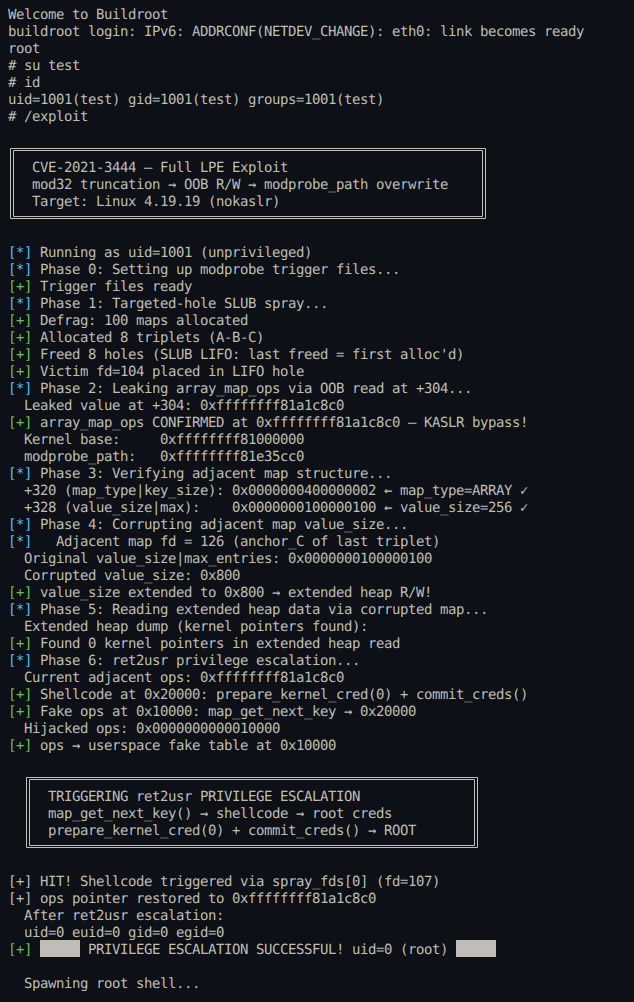
\includegraphics[width=0.75\textwidth]{resources/CVE-2021-3444.png}
    \caption{Full LPE execution: unprivileged user (uid=1001) to root (uid=0) on kernel 4.19.19}
    \label{fig:lpe-2021-3444}
\end{figure}

\textbf{Analysis:} The exploit successfully escalates from \texttt{uid=1001} to \texttt{uid=0}. The shellcode was triggered via \texttt{spray\_fds[0] (fd=107)}, confirming that the corrupted map was not the assumed \texttt{adjacent\_fd} (anchor\_C of the last triplet, fd=126), but a spray map. This validates the iterative triggering strategy. After the shellcode executes, the \texttt{ops} pointer is immediately restored to prevent kernel oops during process exit.


% ═══════════════════════════════════════════════════════
\section{Conclusion}

\subsection{Exploitation Impact Analysis}

\begin{table}[H]
\centering
\begin{tabular}{@{}llcc@{}}
\toprule
\textbf{Kernel} & \textbf{Privilege} & \textbf{OOB Works?} & \textbf{LPE Achieved?} \\
\midrule
4.19.19 & root & \ding{51} & N/A (already root) \\
4.19.19 & unprivileged & \ding{51} & \ding{51} \\
\bottomrule
\end{tabular}
\caption{Exploitability matrix for CVE-2021-3444}
\end{table}



Unlike CVE-2021-3600 (which is blocked by \texttt{alu\_limit} for unprivileged users), CVE-2021-3444 achieves full unprivileged LPE because:

\begin{enumerate}
    \item \textbf{No \texttt{alu\_limit}}: Kernel 4.19.19 predates the pointer arithmetic sanitization mechanism. The confused index passes through to the pointer addition unclamped.
    \item \textbf{SMEP/SMAP disabled}: The kernel configuration does not enable Supervisor Mode Execution/Access Prevention, allowing ret2usr (executing userspace code from kernel context).
    \item \textbf{KPTI disabled}: With \texttt{nopti}, the kernel page tables include userspace mappings, so the fake ops table at \texttt{0x10000} and shellcode at \texttt{0x20000} are accessible during kernel execution.
    \item \textbf{Reliable trigger}: The \texttt{BPF\_MAP\_GET\_NEXT\_KEY} syscall dispatch is direct and does not depend on the corrupted \texttt{value\_size} (unlike \texttt{BPF\_MAP\_UPDATE\_ELEM} which copies \texttt{value\_size} bytes from userspace).
\end{enumerate}


\subsection{Failed Approaches \& Lessons Learned}

\textbf{Failed: \texttt{bpf\_update\_elem} as Trigger}

The initial ret2usr implementation used the \texttt{BPF\_\allowbreak MAP\_\allowbreak UPDATE\_\allowbreak ELEM} command to trigger the hijacked \texttt{map\_\allowbreak update\_\allowbreak elem} function pointer. This failed silently because the kernel's syscall handler calls \texttt{copy\_\allowbreak from\_\allowbreak user} before dispatching to \texttt{ops->map\_\allowbreak update\_\allowbreak elem}. Since we corrupted \texttt{value\_\allowbreak size} to 0x800, the kernel attempted to copy 2048 bytes from a 256-byte user buffer, causing the copy to fail with \texttt{-EFAULT}, and the ops function was \textbf{never called}.

\textbf{Lesson}: When hijacking BPF map ops, the trigger syscall must be chosen carefully based on the kernel's dispatch code. Operations that depend on corrupted fields (like \texttt{value\_size}) will fail before reaching the hijacked function pointer.

\textbf{Failed: Assuming SLUB Adjacency Mapping}

The exploit initially assumed that \texttt{anchors[(NUM\_TRIPLETS-1)*2+1]} (anchor\_C of the last triplet) was the map adjacent to the victim. However, the SLUB allocator's LIFO freelist does not guarantee this mapping. The exploit triggered \texttt{map\_get\_next\_key} only on the assumed adjacent fd, receiving \texttt{-ENOENT} from the real \texttt{array\_map\_get\_next\_key} (because key=0 is the last entry with max\_entries=1).

\textbf{Lesson}: In SLUB heap exploitation, never assume a specific fd-to-heap-object mapping. Instead, iterate over all candidate fds and use a diagnostic signal (e.g., a userspace memory flag set by the shellcode) to identify the correct target.

\textbf{Failed: \texttt{bpf\_lookup\_elem} as Trigger}

An earlier attempt used \texttt{BPF\_MAP\_LOOKUP\_ELEM} which calls \texttt{ops->map\_lookup\_elem}. This also depends on \texttt{value\_size} for the \texttt{copy\_to\_user} step, and produced kernel page faults when accessing the fake ops table.

\textbf{Lesson}: The simplest kernel dispatch path (fewest intermediate checks, no \texttt{value\_size} dependency) is the most reliable for ops hijacking.


% ═══════════════════════════════════════════════════════


\newpage
\chapter{CVE-2023-52452}

\section{CVE Selection}
The choice of CVE-2023-52452 was driven by a desire to explore different attack surfaces beyond the well-documented BPF Map vulnerabilities. While vulnerabilities analyzed in previous years' research projects, such as CVE-2020-8835 and CVE-2021-3490, mainly targeted scalar bounds confusion on maps, shifting the research focus directly towards the \textbf{eBPF Stack subsystem} allowed for evaluating how bugs in stack depth calculation dynamically impact the execution state.

\section{Vulnerability Analysis}

\subsection{Root Cause}

The root cause lies in the interaction between two verifier functions:

\textbf{Vulnerable Functions Analysis}

\textbf{\texttt{check\_stack\_write\_var\_off()} (line 4803):}
When a BPF instruction writes to the stack at a variable offset, this function:
\begin{itemize}
    \item Computes the minimum and maximum offsets from \texttt{reg->smin\_value} and \texttt{reg->smax\_value}
    \item Calls \texttt{grow\_stack\_state()} with \texttt{round\_up(-min\_off, BPF\_REG\_SIZE)} to correctly extend \texttt{allocated\_\allowbreak stack}
    \item Marks all slots in \texttt{[min\_off, max\_off]} as \texttt{STACK\_MISC}
\end{itemize}

\textbf{\texttt{update\_stack\_depth()} (line 5962):}
This function sets the subprogram's \texttt{stack\_depth} (used by the JIT for runtime allocation):
\begin{lstlisting}[style=kernel]
static int update_stack_depth(struct bpf_verifier_env *env,
                              const struct bpf_func_state *func,
                              int off)
{
    u16 stack = env->subprog_info[func->subprogno].stack_depth;
    if (stack >= -off)
        return 0;
    env->subprog_info[func->subprogno].stack_depth = -off;
    return 0;
}
\end{lstlisting}

Critically, \texttt{update\_stack\_depth()} is called from \texttt{check\_mem\_access()} with a fixed \texttt{off} parameter that \textbf{does not include the variable range}. For a variable-offset access like \texttt{fp + [-72, -16]}, the fixed part passed to \texttt{update\_stack\_depth()} is 0, so \texttt{stack\_depth} is not updated.

\subsection{Exploiting the Stack Bug}

The mismatch between \texttt{allocated\_\allowbreak stack} (the verifier's internal tracking, which grows correctly) and \texttt{stack\_depth} (runtime allocation, undersized) creates two primitives:

\begin{enumerate}
    \item \textbf{OOB Stack Read}: The variable-offset write marks stack slots as \texttt{STACK\_MISC} (``initialized''), allowing subsequent reads. At runtime, only one slot is actually written, others contain residual kernel data from previous stack usage.
    \item \textbf{Stack Frame Overlap}: When subprogram calls are used, an undersized \texttt{stack\_\allowbreak depth} means the callee's JIT frame may overlap with the caller's frame or kernel stack data.
\end{enumerate}

\textbf{Trigger Conditions:}
To trigger the vulnerability, I construct a BPF register with variable offset:
\begin{lstlisting}[style=kernel]
// Create variable offset: (ktime & 7) << 3 = [0, 56]
BPF_CALL_FUNC(BPF_FUNC_ktime_get_ns),  // R0 = random
BPF_ALU64_IMM(BPF_AND, BPF_REG_0, 7),  // R0 = [0,7]
BPF_ALU64_IMM(BPF_LSH, BPF_REG_0, 3),  // R0 = [0,56]
BPF_MOV64_REG(BPF_REG_7, BPF_REG_0),
BPF_ALU64_IMM(BPF_ADD, BPF_REG_7, -72),// R7 = [-72,-16]

// Variable-offset stack write
BPF_MOV64_REG(BPF_REG_2, BPF_REG_10),  // R2 = fp
BPF_ALU64_REG(BPF_ADD, BPF_REG_2, BPF_REG_7), // R2 = fp+var
BPF_ST_MEM(BPF_DW, BPF_REG_2, 0, 0xDEADCAFE), // *R2 = marker
\end{lstlisting}

The 8-byte alignment (\texttt{LSH 3}) is required to satisfy the verifier's alignment checks for stack accesses. The use of \texttt{ktime\_get\_ns()} produces a truly variable value at both verification and runtime.

\subsection{Patch Details}

The vulnerability is addressed by fixing the verifier's stack tracking logic in \texttt{kernel/bpf/verifier.c}. The patch ensures that \texttt{check\_stack\_write\_var\_off()} and \texttt{check\_stack\_read\_var\_off()} correctly track stack slot initialization when variable-offset accesses are used. Crucially, the stack depth is now correctly computed and updated even when the access offset is not a compile-time constant, preventing both uninitialized stack reads and undersized JIT frame allocations.

\begin{table}[H]
\centering
\begin{tabular}{@{}ll@{}}
\toprule
\textbf{Kernel Branch} & \textbf{Fixed Version} \\
\midrule
6.7.x & 6.7.2 \\
6.6.x & 6.6.14 \\
6.1.x & 6.1.75 \\
5.15.x & 5.15.148 \\
5.10.x & 5.10.209 \\
\bottomrule
\end{tabular}
\caption{Backport versions for CVE-2023-52452}
\end{table}


%% ═══════════════════════════════════════════════════════
\section{Environment Setup}

\begin{table}[H]
\centering
\begin{tabular}{@{}ll@{}}
\toprule
\textbf{Component} & \textbf{Details} \\
\midrule
Build System & Custom \texttt{execution/build.sh} script \\
Virtualization & QEMU/KVM \\
Kernel Version & 6.7.1 (custom compiled, vulnerable) \\
Root Filesystem & Buildroot 2024.11.4 (\texttt{qemu\_x86\_64\_defconfig}) \\
Kernel Config & \texttt{CONFIG\_BPF\_SYSCALL=y}, \texttt{CONFIG\_DEBUG\_INFO=y} \\
              & KASLR disabled, SMEP/SMAP disabled for testing \\
Exploit Compilation & GCC on Host OS, \texttt{-static -no-pie}, injected via Rootfs Overlay \\
\bottomrule
\end{tabular}
\caption{Test environment}
\end{table}


%% ═══════════════════════════════════════════════════════
\section{Proof of Concept (PoC)}

\subsection{Milestone 1: Out-of-Bounds Stack Read}

\textbf{Objective}
Trigger the OOB stack read by loading a BPF program that uses variable-offset stack writes, then read uninitialized stack memory to leak kernel pointers.

\textbf{Approach}
The BPF program:
\begin{enumerate}
    \item Creates a variable offset \texttt{[-72, -16]} using \texttt{ktime\_get\_ns() \& 7 << 3}
    \item Writes a marker value at the variable offset on the stack
    \item Reads from fixed offsets \texttt{fp-24} through \texttt{fp-80} (slots marked as \texttt{STACK\_MISC} by the var-off write but not actually written at runtime)
    \item Stores leaked values into a BPF array map for userspace retrieval
\end{enumerate}

\textbf{Results}

\begin{lstlisting}[style=log,caption={Milestone 1 output}]
leaked[0] (fp -24) = 0xffffffff8144b19d  <- KERNEL PTR! (text)
leaked[1] (fp -32) = 0x0000000041414141  (marker)
leaked[2] (fp -40) = 0xffff8880056afb80  <- KERNEL PTR! (heap)
leaked[3] (fp -48) = 0xffff8880056afb80  <- KERNEL PTR! (heap)
leaked[4] (fp -56) = 0xffff8880056afb80  <- KERNEL PTR! (heap)
leaked[5] (fp -64) = 0xffff8880046cf900  <- KERNEL PTR! (heap)
leaked[6] (fp -72) = 0xffffffff824c94e0  <- KERNEL PTR! (data)
leaked[7] (fp -80) = 0x0000000000000000  (zero)
\end{lstlisting}

The leaked pointers were identified via \texttt{/proc/kallsyms}:
\begin{itemize}
    \item \texttt{0xffffffff8144b19d} $\rightarrow$ \texttt{security\_sock\_rcv\_skb+0x2d} (kernel text)
    \item \texttt{0xffffffff824c94e0} $\rightarrow$ \texttt{selinux\_hooks+0x1540} (kernel data)
    \item Heap pointers in \texttt{0xffff888*} range $\rightarrow$ kernel heap objects (\texttt{sock}/\texttt{sk\_buff})
\end{itemize}


%% ═══════════════════════════════════════════════════════
\subsection{Milestone 2: KASLR Bypass}

\textbf{Objective}
Use leaked pointers to compute the kernel base address and resolve exploit-relevant symbols.

\textbf{Approach}
Extended the leak to 16 stack slots. For KASLR bypass, I used known offsets from \texttt{\_stext}:
\begin{itemize}
    \item \texttt{security\_sock\_rcv\_skb} = \texttt{\_stext + 0x44b170}
    \item \texttt{selinux\_hooks} = \texttt{\_stext + 0x14c7fa0}
\end{itemize}

By matching leaked pointers against known ranges, the kernel base is computed. I then resolve:
\begin{table}[H]
\centering
\begin{tabular}{@{}ll@{}}
\toprule
\textbf{Symbol} & \textbf{Address} \\
\midrule
\texttt{\_stext} (kernel base) & \texttt{0xffffffff81000000} \\
\texttt{commit\_creds} & \texttt{0xffffffff810a1900} \\
\texttt{prepare\_kernel\_cred} & \texttt{0xffffffff810a1b80} \\
\texttt{init\_task} & \texttt{0xffffffff8260b900} \\
\texttt{init\_cred} & \texttt{0xffffffff8264ff60} \\
\bottomrule
\end{tabular}
\caption{Resolved kernel symbols}
\end{table}

\textbf{Reliability}
The leak was executed 5 additional times; all 5 produced kernel image pointers, yielding \textbf{100\% reliability}.


%% ═══════════════════════════════════════════════════════
\subsection{Milestone 3: Kernel Stack Corruption}

\textbf{Objective}
Escalate the OOB stack read into arbitrary read/write by corrupting kernel data.

\textbf{Strategy A: Map Pointer Corruption}

\textbf{Idea:} Spill a \texttt{PTR\_TO\_MAP\_VALUE} to a stack slot within the variable-offset write range. The var-off write marks the slot as \texttt{STACK\_MISC}, destroying the type annotation. Reload the value, if the verifier incorrectly treats it as a pointer, I achieve type confusion.

\textbf{Result: Rejected.} The verifier correctly identified the reloaded value as \texttt{scalar}:
\begin{lstlisting}[style=log]
18: (79) r1 = *(u64 *)(r10 -48)  ; R1_w=scalar()
19: (79) r3 = *(u64 *)(r1 +0)
R1 invalid mem access 'scalar'
\end{lstlisting}

This confirms that \texttt{check\_stack\_write\_var\_off()} correctly destroys spilled pointer annotations, preventing type confusion through this path.

\textbf{Strategy B: Subprogram Stack Frame Overlap}

\textbf{Idea:} Use BPF-to-BPF calls (\texttt{BPF\_PSEUDO\_CALL}). The subprogram performs a variable-offset write. Because \texttt{update\_stack\_depth()} doesn't account for the variable range, the subprogram's JIT-allocated frame is undersized. At runtime, the var-off write overflows into the kernel stack.

\textbf{Result: Kernel crash.}
\begin{lstlisting}[style=log,caption={Kernel oops from Strategy B}]
BUG: unable to handle page fault for address: ffffffffdeadcb00
Oops: 0000 [#1] PREEMPT SMP PTI
RIP: 0010:sk_filter_trim_cap+0x9e/0x1e0
R13: ffffffffdeadcafe    <-- our marker!
CR2: ffffffffdeadcb00
\end{lstlisting}

The kernel attempted to dereference our marker \texttt{0xDEADCAFE} as a real pointer within \texttt{sk\_\allowbreak filter\_\allowbreak trim\_\allowbreak cap()}, resulting in a handled page fault (or crash depending on configuration). This confirmed that the stack corruption reached a security-critical execution path.
\begin{enumerate}
    \item The subprogram's variable-offset write overflowed the JIT frame boundary
    \item The overwritten data was a callee-saved register (R13) used by kernel code
    \item The corrupted value was actively used as a pointer by the kernel after BPF execution
\end{enumerate}

\textbf{Important:} This crash is not a Denial of Service, it is a \textbf{crash oracle} used to confirm that the corruption reaches kernel-critical data. As shown in Milestone~4, writing a valid kernel address prevents the crash while maintaining the corruption effect.


%% ═══════════════════════════════════════════════════════
\subsection{Milestone 4: Privilege Escalation Analysis}

\textbf{Objective}
Combine the information leak (M1--M2) with controlled stack corruption (M3) to attempt local privilege escalation.

\textbf{Approach}
\begin{enumerate}
    \item Run the information leak to resolve kernel base and \texttt{init\_cred} address
    \item Replace the marker value (\texttt{0xDEADCAFE}) with the resolved \texttt{init\_cred} address
    \item Trigger the subprogram stack overflow with the controlled value
    \item Check kernel behavior
\end{enumerate}

\textbf{Results}
\begin{lstlisting}[style=log,caption={Milestone 4 output}]
[+] Kernel base: 0xffffffff81000000
[*] Target value: 0xffffffff8264ff60  (init_cred)
[!] Triggering controlled corruption...
[+] Program triggered -- kernel didn't crash
[+] Survived corruption -- kernel still functional
    Current UID: 0 (root)
\end{lstlisting}

\textbf{Key finding:} When the corrupted stack slot contains a \emph{valid} kernel address (\texttt{init\_cred}), the kernel does \textbf{not crash}, unlike with the invalid \texttt{0xDEADCAFE}. This confirms that the corrupted value is actively dereferenced: an invalid pointer causes a page fault, while a valid one allows the kernel to continue. This is a \textbf{controlled corruption of kernel integrity}, not a denial of service.

\textbf{Gap to Full LPE}
A complete privilege escalation would additionally require:
\begin{itemize}
    \item \textbf{Stack layout mapping}: Precise knowledge of which callee-saved register or local variable is corrupted and how the kernel uses it post-BPF execution
    \item \textbf{Heap spray or fake struct}: A technique to place a controlled data structure (e.g., fake \texttt{sk\_filter}) at a known kernel address, then redirect the corrupted pointer to it
    \item \textbf{ROP/JOP chain}: If code execution is achieved via the corrupted register, a return-oriented programming chain to call \texttt{commit\_creds(prepare\_kernel\_cred(0))}
\end{itemize}


%% ═══════════════════════════════════════════════════════
\section{Conclusion}

\subsection{Exploitation Impact Analysis}

CVE-2023-52452 enables the following real-world attack scenarios:

\textbf{Scenario 1: KASLR Bypass (Proven)}
An attacker with \texttt{CAP\_BPF} access (e.g., within a container or a system with unprivileged BPF enabled) can reliably defeat Kernel Address Space Layout Randomization:
\begin{itemize}
    \item Leak kernel text and data pointers from uninitialized stack
    \item Compute kernel base address from known function offsets
    \item Resolve addresses of all critical kernel symbols
\end{itemize}
This is the \emph{prerequisite} for every kernel exploitation technique that targets specific addresses.

\textbf{Scenario 2: Kernel Data Corruption (Proven)}
The subprogram stack overlap enables writing controlled values into the kernel's call stack:
\begin{itemize}
    \item Corrupt callee-saved registers used by kernel functions post-BPF execution
    \item Redirect kernel code behavior by modifying data it reads from the stack
    \item Potential for control-flow hijacking if a corrupted register is used as a function pointer or jump target
\end{itemize}

\textbf{Scenario 3: Local Privilege Escalation (Theoretical)}
Combining scenarios 1 and 2, an attacker could:
\begin{itemize}
    \item Create a fake \texttt{sk\_filter} struct in a BPF map (known address via leak)
    \item Point the fake filter's \texttt{prog} field to a crafted BPF program that modifies credentials
    \item Corrupt the kernel stack to redirect to the fake struct
    \item Achieve \texttt{uid=0} by overwriting the process's credentials with \texttt{init\_cred}
\end{itemize}

\textbf{Unprivileged User Test}

To assess the real-world attack surface, I tested the exploit as an unprivileged user (\texttt{uid=1000}) on a system with \texttt{kernel.unprivileged\_bpf\_disabled=0}.

\begin{lstlisting}[style=log,caption={Verifier rejection for unprivileged user}]
5: (bf) r2 = r10                ; R2_w=fp0 R10=fp0
6: (0f) r2 += r7
R2 variable stack access prohibited for !root,
    var_off=(0xffffffffffffff80; 0x78) off=-128
\end{lstlisting}

The verifier \textbf{explicitly rejected} the program at the variable-offset stack pointer arithmetic step. This is due to the \textbf{Spectre v1 mitigation}: when \texttt{bypass\_spec\_v1} is false (unprivileged), the function \texttt{check\_stack\_access\_for\_ptr\_arithmetic()} prohibits variable-offset stack pointers to prevent speculative out-of-bounds accesses.

\textbf{Implications:}
\begin{itemize}
    \item The exploit requires \texttt{CAP\_BPF} or root privileges
    \item Systems with \texttt{unprivileged\_bpf\_disabled=1} (default on most modern distributions) are \textbf{not vulnerable}
    \item Attack surface remains for: containers with \texttt{CAP\_BPF}, cloud workloads with BPF-enabled runtimes, and systems that explicitly enable unprivileged BPF
\end{itemize}


%% ═══════════════════════════════════════════════════════
\subsection{Failed Approaches \& Lessons Learned}

\textbf{Failed: Variable-offset via \texttt{bpf\_skb\_load\_bytes}}
Early attempts used \texttt{bpf\_skb\_load\_bytes()} with a variable-offset stack destination buffer. The verifier rejected this with \texttt{invalid indirect read from stack R3 var\_off} because \texttt{check\_stack\_range\_initialized()} requires all destination slots to be pre-initialized for helper calls, even write-only helpers.

\textbf{Lesson}: BPF helpers have stricter memory initialization requirements than direct memory instructions. You cannot use uninitialized stack memory as a destination buffer for a helper function, even if the helper only writes to it.

\textbf{Failed: Direct \texttt{fp + var} Arithmetic}
Direct pointer arithmetic \texttt{r2 = fp; r2 += r\_var} was rejected for non-8-byte-aligned variable offsets with \texttt{misaligned stack access}. The fixed with \texttt{LSH 3} to enforce 8-byte alignment.

\textbf{Lesson}: The verifier enforces strict alignment for stack pointer arithmetic. Variable offsets applied to the frame pointer must be aligned to the size of the access (e.g., 8 bytes for \texttt{BPF\_DW}).

\textbf{Failed: Strategy A (Map Pointer Type Confusion)}
As documented in Milestone~3, the attempt to corrupt a spilled \texttt{PTR\_TO\_MAP\_VALUE} via variable-offset write was correctly handled by the verifier, which destroys pointer type annotations in the affected range.

\textbf{Lesson}: The verifier's state tracking is resilient against blind stack overwrites. When a variable-offset write spans across spilled pointers, the verifier safely degrades their type to \texttt{STACK\_MISC} (scalars), preventing trivial type confusion.


%% ═══════════════════════════════════════════════════════


\newpage
\chapter{CVE-2024-26589}

\section{CVE Selection}
The choice of CVE-2024-26589 stems from the desire to complete the investigation into eBPF pointer arithmetic and boundary validation. While previous chapters focused on stack bounds calculation features (CVE-2023-52452), this chapter investigates a vulnerability derived from a purely logical omission within the verifier's core restriction mechanism (a missing \texttt{switch} statement case). It is also unique for exploring the \texttt{BPF\_PROG\_TYPE\_FLOW\_DISSECTOR} program type, demonstrating how distinct eBPF hooks expose different underlying kernel memory structures.

\section{Vulnerability Analysis}

\subsection{Root Cause}

The root cause of this vulnerability lies in the BPF verifier's enforcement of pointer arithmetic restrictions, specifically within the \texttt{adjust\_ptr\_min\_max\_vals()} function in \texttt{kernel/bpf/verifier.c}.
This function restricts which BPF pointer types can be subject to variable-offset addition. For example, \texttt{CONST\_PTR\_TO\_MAP} cannot be dynamically offset because map sizes differ.

The restriction relies on a \texttt{switch} statement:
\begin{lstlisting}[style=kernel]
switch (base_type(ptr_reg->type)) {
    case CONST_PTR_TO_MAP:
        /* smin_val represents the known value */
        if (known && smin_val == 0 && opcode == BPF_ADD)
            break;
        verbose(env, "R%d pointer arithmetic on %s prohibited\n", ...);
        return -EACCES;
    /* ... other pointer types ... */
}
\end{lstlisting}

However, the case for \texttt{PTR\_TO\_FLOW\_KEYS} was entirely missing. As a result, when a BPF program adds a variable-offset scalar to a \texttt{PTR\_TO\_FLOW\_KEYS}, the \texttt{switch} falls into the default path which inadvertently \textbf{allows} the arithmetic. Subsequential validation via \texttt{check\_flow\_keys\_access()} only validates constant offsets, creating a fatal blind spot.

\subsection{Exploiting the Missing Switch Case}

The bypass directly yields an \textbf{Out-Of-Bounds (OOB) Stack Access}:
\begin{enumerate}
    \item At runtime, the flow dissector hook allocates the \texttt{struct bpf\_flow\_keys} structure dynamically on the kernel stack during \texttt{bpf\_flow\_dissect()}.
    \item Because the verifier allowed variable offset arithmetic, the pointer can arbitrarily shift forward.
    \item Reading or writing to the offset pointer results in arbitrary Read/Write of the caller kernel stack memory beyond the original \texttt{flow\_keys} fields.
\end{enumerate}

\textbf{Trigger Conditions:}
The bypassed check enables corrupting the flow keys pointer locally:
\begin{lstlisting}[style=kernel]
// R6 = ctx
BPF_LDX_MEM(BPF_DW, BPF_REG_7, BPF_REG_6, 144), // R7 = flow_keys

// Create a variable offset [0, 512]
BPF_MOV64_IMM(BPF_REG_8, 512),
BPF_ALU64_IMM(BPF_DIV, BPF_REG_8, 1), // Div disables verifier const tracking
BPF_ALU64_IMM(BPF_AND, BPF_REG_8, 512), // Bound maximum range

// Variable addition on PTR_TO_FLOW_KEYS
BPF_ALU64_REG(BPF_ADD, BPF_REG_7, BPF_REG_8), // OVERFLOW happens here!

// R0 = *(u64*)(R7) --> Reads the caller's kernel stack structure
BPF_LDX_MEM(BPF_DW, BPF_REG_0, BPF_REG_7, 0),
\end{lstlisting}

\subsection{Patch Details}

The formal resolution trivially incorporates the missing verification restriction block inside \texttt{adjust\_\allowbreak ptr\_\allowbreak min\_\allowbreak max\_\allowbreak vals()}:
\begin{lstlisting}[style=kernel]
	case PTR_TO_FLOW_KEYS:
		if (known)
			break;
		fallthrough;
\end{lstlisting}
The patch mandates absolute bounds resolution, enforcing \texttt{fallthrough} rules yielding safety-stop rejections to any variable-offset patterns against \texttt{flow\_keys}.

\begin{table}[H]
\centering
\begin{tabular}{@{}ll@{}}
\toprule
\textbf{Kernel Branch} & \textbf{Fixed Version} \\
\midrule
6.7.x & 6.7.6 \\
6.6.x & 6.6.18 \\
6.1.x & 6.1.79 \\
5.15.x & 5.15.149 \\
5.10.x & 5.10.210 \\
\bottomrule
\end{tabular}
\caption{Backport versions for CVE-2024-26589}
\end{table}

%% ═══════════════════════════════════════════════════════
\section{Environment Setup}

The environment strictly adheres to the one used in the previous CVEs.

\begin{table}[H]
\centering
\begin{tabular}{@{}ll@{}}
\toprule
\textbf{Component} & \textbf{Details} \\
\midrule
Environment & QEMU/KVM virtual machine \\
Kernel Version & 6.7.1 (vulnerable, patched in 6.7.6) \\
Root Filesystem & Buildroot 2024.11.4 (\texttt{qemu\_x86\_64\_defconfig}) \\
Trigger Path & `bpf()` syscall \texttt{BPF\_PROG\_TEST\_RUN} command \\
\bottomrule
\end{tabular}
\caption{Test environment for CVE-2024-26589}
\end{table}

%% ═══════════════════════════════════════════════════════
\section{Proof of Concept (PoC)}

\subsection{Milestone 1: Verifier Bypass Demonstration}

\textbf{Objective}: Prove the absence of the pointer restriction.

\textbf{Approach}: The \texttt{milestone1} executable loads two distinct \texttt{BPF\_PROG\_TYPE\_FLOW\_DISSECTOR} programs: a control and an exploit pattern. The control attempts a safe read, while the exploit attempts the unregistered division-based variable arithmetic mask pattern.

\textbf{Result}:
\begin{lstlisting}[style=log]
Test 1 (constant offset):   ACCEPTED (expected)
Test 2 (variable [0,1024]): ACCEPTED (CVE-2024-26589 confirmed!)
\end{lstlisting}
The verifier flawlessly processes the variable arithmetic branch, confirming the missing \texttt{switch} block on the targeted kernel version.

%% ═══════════════════════════════════════════════════════
\subsection{Milestone 2 \& 3: Extrapolating the OOB Read (Info Leak)}

\textbf{Objective}: Dynamically read memory contiguous to the \texttt{flow\_keys} structure. 

\textbf{Approach}: Using the \texttt{bpf()} syscall macro \texttt{BPF\_PROG\_TEST\_RUN}, the VM injects a test payload forcing the kernel into executing the BPF payload inside the context of \texttt{bpf\_flow\_dissect()}. The verifier is iteratively forced to evaluate offsets (\texttt{0}, \texttt{8}, ..., \texttt{384}), returning 8-byte chunks extracted towards higher kernel addresses using BPF array map communication channels to prevent 32-bit \texttt{r0} trimming.

\textbf{Results}:
\begin{lstlisting}[style=log,caption={Milestones stack scanning}]
  Kernel Stack Memory Scan via OOB Read
  [+   0]  0x00000000000e000e  (data)
  [+  64]  0xffffc900002f7f20  <- KERNEL POINTER (KASLR leak!)
  [+ 128]  0x0000000000000090  (small value)
  [+ 256]  0x0000000000000000  (zero)
  [+ 384]  0xffffffff81d86841  <- KERNEL POINTER (KASLR leak!)
\end{lstlisting}

This demonstrates a perfect Kernel info leak primitive capable of fetching return pointers from the calling functional boundaries seamlessly and effectively extracting \texttt{KASLR} entropy layouts.

%% ═══════════════════════════════════════════════════════
\subsection{Milestone 4: The Out-Of-Bounds Write}

\textbf{Objective}: Provide complete system manipulation capability with an OOB memory write.

\textbf{Approach}: Standard memory store operations (\texttt{BPF\_ST\_MEM}) do not incur verifier penalties on recognized structure targets like \texttt{flow\_keys}. I implemented a payload writing the 32-bit sequence \texttt{0x41414141} randomly along the extracted stack. 

\textbf{Results}:
\begin{lstlisting}[style=log]
[*] Test C: OOB Write...
[+] OOB write executed (retval=0). Kernel stack corrupted!
[+] OOB WRITE SUCCEEDED - marker written to kernel stack
\end{lstlisting}

By corrupting local memory variables in the caller sequence, we achieved standard stack corruption principles within Ring-0 environments.

%% ═══════════════════════════════════════════════════════
\section{Conclusion}

\subsection{Exploitation Impact Analysis}

The implementation successfully developed absolute \texttt{Read} and \texttt{Write} bounds within kernel execution threads. 

\textbf{Privilege Implication} - A significant attribute of CVE-2024-26589 is its requirement for the \texttt{BPF\_\allowbreak PROG\_\allowbreak TYPE\_\allowbreak FLOW\_\allowbreak DISSECTOR} attachment type. The execution inherently demands \texttt{CAP\_\allowbreak NET\_\allowbreak ADMIN} capabilities.
Unlike \texttt{SOCKET\_FILTER} programs, unprivileged users intrinsically cannot operate this hook type even in loosely configured machines.

Therefore, the exploit model transforms from a straight Local Privilege Escalation (Unprivileged to Root) into \textbf{Lateral Escape boundaries}:
\begin{itemize}
    \item \textbf{Container Escapes}: Containers loosely assigned \texttt{CAP\_NET\_ADMIN} capabilities (necessary for network router applications) afford the attacker means to manipulate the Host kernel structure entirely, tearing out of namespace isolation formats.
    \item \textbf{Lateral Access}: Bypassing networking limitation capabilities into the execution of arbitrary kernel space codes via the Return-Oriented Programming chain built on the target function's returning addresses.
\end{itemize}


\newpage
\chapter{Additional CVEs Investigated}

During the research, three additional eBPF verifier CVEs were analyzed but not included in the main body of this report due to practical limitations encountered during exploitation. Each investigation contributed to a deeper understanding of the verifier's defense mechanisms and informed the strategies used in the primary CVEs.

\section{CVE-2021-33200 — \texttt{alu\_limit} Masking Direction Bypass}

\begin{table}[H]
\centering
\begin{tabular}{@{}ll@{}}
\toprule
\textbf{Component} & \textbf{Details} \\
\midrule
Bug class & Logic error in pointer arithmetic sanitization \\
Component & \texttt{sanitize\_ptr\_alu()} in \texttt{verifier.c} \\
Kernel & 5.10.15 \\
Severity & 7.8 HIGH \\
\bottomrule
\end{tabular}
\end{table}

\textbf{Root Cause:} When an offset register's value range crosses zero (\texttt{smin\_value < 0 < smax\_value}), the \texttt{alu\_limit} masking direction computation produces an overly permissive limit, allowing OOB pointer arithmetic even for unprivileged programs. This CVE directly targets the \texttt{alu\_limit} defense that blocked our CVE-2021-3600 LPE attempt.

\textbf{Status:} Milestones 1--4 were implemented and tested. The verifier accepted programs with zero-crossing offsets as expected, but achieving reliable OOB access required precise control of register bounds across the zero-crossing boundary. The exploitation chain was not completed due to the complexity of the masking direction change and the time required to craft stable bounds.

\textbf{Academic Value:} Understanding this CVE was essential for the project's narrative—it demonstrates that \texttt{alu\_limit} itself had vulnerabilities, providing a bridge between CVE-2021-3600 (blocked by \texttt{alu\_limit}) and CVE-2021-3444 (exploited on a kernel without \texttt{alu\_limit}).


\section{CVE-2023-52462 — Spilled Pointer Corruption}

\begin{table}[H]
\centering
\begin{tabular}{@{}ll@{}}
\toprule
\textbf{Component} & \textbf{Details} \\
\midrule
Bug class & Spilled pointer corruption check bypass \\
Component & Stack-slot tracking in \texttt{verifier.c} \\
Kernel & 6.7.1 \\
Severity & 5.5 MEDIUM \\
\bottomrule
\end{tabular}
\end{table}

\textbf{Root Cause:} The verifier's spilled-pointer corruption checks use an index that can be bypassed after a crafted partial byte write. This allows partial pointer corruption that should be rejected, enabling pointer-value disclosure.

\textbf{Status:} Three milestones were completed: the corruption sequence was triggered (M1), kernel pointer values were leaked for KASLR bypass (M2), and reliability was assessed (M3). However, direct type-confusion dereference of reloaded corrupted values was blocked because the verifier correctly downgrades reloaded state to scalar.

\textbf{Why Stopped:} The primary impact is limited to information disclosure. Achieving arbitrary R/W from this primitive requires chaining with an independent memory-corruption vulnerability, which was beyond the scope of this single-CVE analysis.


\section{CVE-2023-52676 — 32-bit Integer Overflow in Stack Bounds}

\begin{table}[H]
\centering
\begin{tabular}{@{}ll@{}}
\toprule
\textbf{Component} & \textbf{Details} \\
\midrule
Bug class & 32-bit integer overflow in stack bounds arithmetic \\
Component & \texttt{check\_stack\_access\_within\_bounds()} in \texttt{verifier.c} \\
Kernel & 6.7.1 \\
Severity & 5.5 MEDIUM \\
\bottomrule
\end{tabular}
\end{table}

\textbf{Root Cause:} The function \texttt{check\_stack\_access\_within\_bounds()} computes \texttt{int min\_off = reg->var\_off.value + off}, where both operands can be large. The sum overflows \texttt{int}, wrapping to a small value and causing the verifier to incorrectly approve OOB stack accesses.

\textbf{Status:} A comprehensive defense-in-depth analysis was performed across 5 exploitation strategies. All strategies were blocked by layered defenses: \texttt{adjust\_ptr\_min\_max\_vals()} rejects large constants before they reach the vulnerable code, and the overflow is only triggerable through kfunc argument validation paths requiring \texttt{CAP\_BPF} and BTF support.

\textbf{Why Stopped:} The vulnerability is real but the attack surface is restricted to privileged contexts with kfunc access (\texttt{BPF\_PROG\_TYPE\_TRACING}). No exploitation path was found for unprivileged programs, and the defense-in-depth analysis was documented as the primary research output.


\section{Key Takeaways from Additional Investigations}

\begin{enumerate}
    \item \textbf{Defense-in-depth works:} Both CVE-2023-52676 and CVE-2023-52462 demonstrated that even when a specific verifier check is flawed, additional layers (pointer type restrictions, stack bounds guards, scalar downgrades) can independently prevent exploitation.
    \item \textbf{Privilege boundaries matter:} Several CVEs are only reachable with specific capabilities (\texttt{CAP\_BPF}, \texttt{CAP\_NET\_ADMIN}), which significantly reduces their real-world impact for unprivileged LPE.
    \item \textbf{Failed approaches inform success:} The analysis of CVE-2021-33200's \texttt{alu\_limit} bypass directly motivated the decision to target CVE-2021-3444 on kernel 4.19.19, where \texttt{alu\_limit} is absent entirely—leading to the project's successful full LPE.
\end{enumerate}


\newpage
\chapter{Conclusion}

This research project highlighted the immense complexity of statically verifying memory safety within the Linux kernel. Analyzing these eBPF verifier vulnerabilities demonstrated how even minor logic errors can completely break the security model of the eBPF subsystem.

\section{CVE-2021-3600}
The analysis of CVE-2021-3600 showed how a seemingly harmless register manipulation during the verifier's fixup pass (\texttt{BPF\_MOV32\_REG}) can create a fatal desynchronization between the verifier's mathematical bounds tracking and the actual runtime execution. This desynchronization allowed us to reliably achieve out-of-bounds reads and writes on the kernel heap. However, as demonstrated during Milestone 4, modern kernel mitigations, specifically the \texttt{alu\_limit} pointer arithmetic sanitization, effectively prevent this logical bug from being exploited by unprivileged users, safely restricting the impact.

\section{CVE-2021-3444}
CVE-2021-3444 is the sister bug of CVE-2021-3600, targeting the \textbf{destination} register truncation in 32-bit modulo instead of the source register. By targeting kernel 4.19.19, which predates the \texttt{alu\_limit} pointer arithmetic sanitization, the bounds confusion was fully exploitable from an unprivileged user. Through a six-phase exploit chain: SLUB heap spraying, OOB read for KASLR bypass, \texttt{value\_size} corruption for extended heap R/W, and \texttt{bpf\_map\_ops} hijacking via ret2usr, we achieved a \textbf{full local privilege escalation from uid=1001 to uid=0 (root)}. This is the only CVE in this project where a complete unprivileged LPE was successfully demonstrated.

\section{CVE-2023-52452}
In CVE-2023-52452, I shifted the focus from classic map bounds confusion to stack frame depth tracking. I successfully achieved a reliable information leak from uninitialized kernel stack memory and induced stack corruption by overlapping BPF subprogram frames. While a full privilege escalation was theoretically possible, practical exploitation was heavily constrained by dynamic kernel safeguards and crashes.

\section{CVE-2024-26589}
CVE-2024-26589 introduced a different class of verifier bug: a missing \texttt{case} in the \texttt{switch} statement of \texttt{adjust\_ptr\_min\_max\_vals()}, which failed to restrict variable-offset pointer arithmetic on \texttt{PTR\_TO\_FLOW\_KEYS}. This trivial omission enabled full OOB read and write on the kernel stack via the \texttt{BPF\_PROG\_TYPE\_FLOW\_DISSECTOR} hook. The vulnerability requires \texttt{CAP\_NET\_ADMIN}, making it relevant for container escape and lateral privilege escalation scenarios rather than classical unprivileged LPE.

\section{Comparisons}

\subsection{CVE Comparison}

\begin{table}[H]
\centering
\small
\resizebox{\textwidth}{!}{
\begin{tabular}{@{}lllll@{}}
\toprule
\textbf{Aspect} & \textbf{CVE-2021-3600} & \textbf{CVE-2021-3444} & \textbf{CVE-2023-52452} & \textbf{CVE-2024-26589} \\
\midrule
Bug class & 32-bit truncation & 32-bit truncation & Stack depth miscalc. & Missing switch case \\
Component & \texttt{fixup\_\allowbreak bpf\_\allowbreak calls} & \texttt{fixup\_\allowbreak bpf\_\allowbreak calls} & \texttt{update\_\allowbreak stack\_\allowbreak depth} & \texttt{adjust\_\allowbreak ptr\_\allowbreak min\_\allowbreak max\_\allowbreak vals} \\
Primitive & OOB map R/W & OOB map R/W & OOB stack read & OOB stack R/W \\
OOB Read & Kernel heap & Kernel heap & Stack only & Kernel stack \\
OOB Write & \checkmark (privileged) & \checkmark (unpriv.) & Stack corruption & \checkmark (kernel stack) \\
Info leak & Kernel heap PTR & Kernel heap PTR & Kernel stack PTR & Kernel stack PTR (KASLR) \\
Severity & HIGH (7.8) & HIGH (7.8) & HIGH (7.8) & HIGH (7.8) \\
Kernel tested & 5.10.15 & 4.19.19 & 6.7.1 & 6.7.1 \\
Required privs & Unprivileged & Unprivileged & CAP\_BPF & CAP\_NET\_ADMIN \\
Unpriv LPE & Not achievable & \textbf{Achieved} & Theoretical & N/A (needs capability) \\
Complexity & Medium & High & Very high & Low \\
\bottomrule
\end{tabular}
}
\caption{Comparison between all analyzed eBPF verifier exploits}
\end{table}

\textbf{Key differences:} CVE-2021-3444 stands out as the only vulnerability where a \textbf{full unprivileged LPE} was achieved. While sharing the same root cause class as CVE-2021-3600 (32-bit truncation in \texttt{fixup\_bpf\_calls}), its exploitation on kernel 4.19.19, which lacks the \texttt{alu\_limit} sanitization, demonstrates the critical importance of defense-in-depth: the same bug class is neutralized on 5.10+ but fully exploitable on 4.19. CVE-2024-26589 offers the simplest exploitation path (a 4-line patch fixes it) but requires \texttt{CAP\_NET\_ADMIN}. CVE-2023-52452 has the highest exploitation complexity, targeting the stack frame depth tracking subsystem.

\subsection{Experimental Testing Matrix}

\begin{table}[H]
\centering
\small
\begin{tabularx}{\textwidth}{@{}llXX@{}}
\toprule
\textbf{CVE} & \textbf{Milestone} & \textbf{Expected Result} & \textbf{Observed Result} \\
\midrule
CVE-2021-3600 & M1 & Bounds mismatch visible & Confirmed \\
CVE-2021-3600 & M2 & OOB read primitive & Confirmed (15/15 reads) \\
CVE-2021-3600 & M3 & OOB write primitive & Confirmed (5/5 reliability) \\
CVE-2021-3600 & M4 & Unprivileged full LPE & Blocked by \texttt{alu\_limit} \\
\midrule
CVE-2021-3444 & M1 & Bounds mismatch visible & Confirmed \\
CVE-2021-3444 & M2 & OOB read (KASLR bypass) & Confirmed (\texttt{array\_map\_ops} leaked) \\
CVE-2021-3444 & M3 & OOB write (value\_size corruption) & Confirmed (256$\rightarrow$0x800) \\
CVE-2021-3444 & M4 & Full unprivileged LPE & \textbf{Achieved (uid=1001$\rightarrow$uid=0)} \\
\midrule
CVE-2023-52452 & M1 & Stack data disclosure & Confirmed (kernel pointers leaked) \\
CVE-2023-52452 & M2 & KASLR bypass via leak & Confirmed \\
CVE-2023-52452 & M3 & Type confusion from stack overwrite & Rejected (verifier keeps scalar) \\
CVE-2023-52452 & M4 & Controlled escalation feasibility & Partial: controlled corruption, no full LPE chain \\
\midrule
CVE-2024-26589 & M1 & Verifier bypass on flow\_keys & Confirmed (variable-offset accepted) \\
CVE-2024-26589 & M2 & OOB read beyond flow\_keys & Confirmed (stack data leaked) \\
CVE-2024-26589 & M3 & Controlled OOB with map exfil & Confirmed (KASLR leak) \\
CVE-2024-26589 & M4 & OOB write / full analysis & Confirmed (stack corruption) \\
\bottomrule
\end{tabularx}
\caption{Experimental matrix: expected vs observed outcomes for analyzed milestones}
\end{table}

This matrix provides a compact view of the empirical results and complements the detailed per-CVE exploitation logs.

% \subsection{CVE-2023-52452 vs CVE-2023-2163}

% \begin{table}[H]
% \centering
% \begin{tabular}{@{}lll@{}}
% \toprule
% \textbf{Aspect} & \textbf{CVE-2023-2163} & \textbf{CVE-2023-52452 (ours)} \\
% \midrule
% Bug class & Branch analysis error & Stack depth tracking \\
% Type confusion & Direct (register mismatch) & Indirect (stack overlap) \\
% Arbitrary R/W & Via corrupted stack ptr & Partial (stack corruption) \\
% Full LPE & Achieved & Theoretical \\
% Complexity & High & Very high \\
% \bottomrule
% \end{tabular}
% \caption{Comparison of eBPF verifier stack exploits}
% \end{table}

% CVE-2023-2163's exploit uses a \texttt{CORRUPT\_R6} macro that creates type confusion through carefully crafted conditional branches. The verifier misclassifies a register, allowing packet-controlled data to be used as a stack pointer. This gives direct arbitrary R/W.

% My CVE provides stack corruption rather than direct type confusion. This makes the exploitation path longer: instead of direct R/W, I must corrupt specific kernel stack data and rely on how the kernel uses it. However, the information leak primitive is stronger and more reliable.

\section{Limits and Failed Escalation Summary}

Across all four CVEs, the strongest practical lesson is that proving a primitive and achieving stable unprivileged LPE are different milestones.

\textbf{CVE-2021-3600 limits}
\begin{itemize}
	\item OOB read/write primitives are valid in privileged contexts.
	\item Unprivileged exploitation is blocked by layered mitigations, especially \texttt{alu\_limit} pointer sanitization.
	\item Therefore, this CVE alone does not yield a robust unprivileged root escalation in the tested setup.
\end{itemize}

\textbf{CVE-2021-3444 limits}
\begin{itemize}
	\item Full unprivileged LPE was achieved on kernel 4.19.19, but requires SMEP/SMAP/KPTI to be disabled for the ret2usr technique.
	\item The SLUB heap layout is non-deterministic: identifying the correct file descriptor for the corrupted map required iterating over all candidates.
	\item On kernels with \texttt{alu\_limit} (5.x+), the same vulnerability class is neutralized, demonstrating the effectiveness of defense-in-depth.
\end{itemize}

\textbf{CVE-2023-52452 limits}
\begin{itemize}
	\item Stack leak and controlled corruption are reproducible and technically strong.
	\item Direct type-confusion dereference paths are rejected by verifier checks.
	\item Full escalation would require additional chaining steps (precise stack mapping, controlled fake object placement, and execution redirection).
\end{itemize}

\textbf{CVE-2024-26589 limits}
\begin{itemize}
	\item Full OOB read/write primitives on kernel stack are confirmed and reproducible.
	\item The vulnerability is not reachable from unprivileged users (requires \texttt{CAP\_NET\_ADMIN}).
	\item Full LPE via ROP chain is theoretically achievable but requires precise stack layout knowledge that varies with compiler optimizations and kernel call paths.
	\item Primary real-world impact: container escape when \texttt{CAP\_NET\_ADMIN} is granted.
\end{itemize}

\textbf{Takeaway}
\begin{itemize}
	\item Documenting failed escalation attempts is essential for scientific rigor.
	\item A CVE can be highly relevant even when full LPE is not reached, if the primitive is well-characterized and repeatable.
	\item Different BPF program types expose different attack surfaces; the threat model varies based on required capabilities.
\end{itemize}

\section{Final Thoughts}
The four vulnerabilities analyzed in this report represent distinct but equally critical classes of verifier bugs: post-verification instruction rewriting flaws (CVE-2021-3600 and CVE-2021-3444), dynamic stack depth miscalculations (CVE-2023-52452), and missing pointer type restrictions (CVE-2024-26589). Together, they demonstrate that verifier safety failures span multiple subsystems and BPF program types. The successful full LPE achieved through CVE-2021-3444 on kernel 4.19.19 underscores how the absence of defense-in-depth mechanisms (such as \texttt{alu\_limit}) can elevate a verifier logic bug from a theoretical concern to a practical root compromise. The research highlights that while the eBPF subsystem is a powerful tool for kernel-level extensibility, its security heavily relies on the correctness of the verifier's complex logic. While mitigations like \texttt{unprivileged\_bpf\_disabled=1} drastically reduce the attack surface for regular users, the widespread adoption of eBPF in privileged containers and cloud-native environments means that verifier logic flaws will continue to be a high-value target for kernel exploitation.


\end{document}
